\documentclass[11pt, a4paper]{article}
\usepackage[utf8]{inputenc} 
\usepackage[left=2cm,text={17cm, 24cm},top=3cm]{geometry}
\usepackage[czech]{babel}
\usepackage{graphicx}

\begin{document}
	\begin{titlepage}
		\begin{center}
			 \textsc{{\Huge Vysoké učení technické v Brně}\\ 
			 \vspace{8.5pt}{\huge Fakulta informačních technologií}}\\
			\vspace{\stretch{0.382}}
			{\LARGE Formální jazyky a překladače\\}
				\vspace{5pt}{\Huge Dokumentace ke skupinovému projektu IFJ a IAL}\\
				\vspace{2pt}{\Large Tým 47, varianta I}
			\vspace{\stretch{0.618}}\\
		\end{center}
		{\small Jakub Zich (vedoucí) - 25\% \emph{xzichj00} \hfill \\
		Patrícia Hudecová - 25\% \emph{xhudec30} \hfill \\
		Ondřej Marek - 25\% \emph{xmarek67} \hfill\\
		Tomáš Willaschek - 25\% \emph{xwilla00} \hfill }
	
	\end{titlepage}	
   
\tableofcontents
\cleardoublepage
\thispagestyle{empty}  

       
 
\section{Úvod} 

Dokumentácia popisuje implementáciu prekladača imperatívneho jazyka IFJ17
	\section{Struktura projektu}
	
	\subsection{Lexikální analyzátor}
Lexikálny analyzátor (scanner) načítava postupnosť znakov (lexém) zo štandardného vstupu a spracováva ich po jednom  pomocou konečného automatu. Konečný automat je naimplementovaný pomocou príkazu switch  (v jazyku C), ktorý je súčasťou funkcie getNextToken. [\ref{ka}]


Komentáre a biele znaky sú spracovávané, ale nikam sa neukladajú po ich spracovaní scanner pokračuje v spracovávaní ďalších znakov. Do štruktúry sa ukladajú identifikátory, kľúčové slova, rezervované kľúčové slová,  čísla (celé, desatinné a v exponenciálnom tvare), reťazcové literály, operátory a niektoré znaky ako napríklad zátvorky a podobne. Tokeny sú na ďalšie spracovanie posielané do syntaktického analyzátora. 

	\subsection{Tabulka symbolů}
    Tabulka symbolů je implementována v podobě binárního stromu. Funkce pro vyhledáváni jsou programovány iterativně, protože rekurzivní přístup by byl při větším počtu položek náročný na paměť. [\ref{symtable}]
		
	
         

	\subsection{Syntaktický analyzátor}
	Syntaktický analyzátor (dále jen SA) pracuje na základě trojrozměrného pole, které reprezentuje LL-gramatiku[\ref{ll}]. První rozměr jsou jednotlivé neterminály, druhý všechny možné pravidla pro jeden neterminál a třetí je jedno pravidlo vložené do pole.
	
		Tyto pravidla se aplikují od zadu na zásobník. Aplikace je prováděna dle precedenční analýzy shora dolů - neterminál na vrcholu zásobníku se rozloží podle terminálu na vstupu. 
		
		SA získává tokeny (terminály) voláním lexikálního analyzátoru. Token se následně porovná s vrcholem zásobníku a když se čísla nerovnají, jedná se o syntaktickou chybu.
		
		Tato konkrétní SA musí rozpoznávat, zda je daný výraz funkce, či skutečný výraz. Proto je objem praviděl poněkud rozsáhlejší. 
		
		Kdykoli, když mý být zpracován výraz, volá se spaciální funkce obsažaná přímo v SA, která konvertuje jednotlivé tokeny na dohodnutý string, který následně pošle precedenční analýze ke skontrolování. 
		Kód se ukládá token po tokenu do struktury, která následně slouží pro kontrolu sémantiky a generování kódu. Při získání tokenu EOL se zkontroluje sémantika aktuálního řádku, a pokud je správná, spustí se generování kódu.

		

\subsection{Precedenční analýza}

Precedenční analýza je volaná ze syntaktické. Pokud syntaktická analýza najde v kódu výraz, zavolá precedenční, která ho zkontroluje a vrátí syntaktické příslušnou návratovou hodnotu podle toho, zda je výraz syntakticky správně, nebo ne.

Naše verze precedenční analýzy nepracuje s jednotlivými tokeny, které posílá lexikální analyzátor, ale pouze s textovým řetězcem. Všechny identifikátory, ať už se v kódu jmenují jakkoli, jsou poslány precedenčnímu analyzátoru jako i. Tedy syntaktický analyzátor, který má přístup k tokenům, a pozná, kde je začátek a konec výrazu, načte příslušné tokeny, vytvoří z nich string, kde změní jména proměnných na i, a pošle string ke kontrole precedenčnímu. Precedenční vrátí pouze 0, 2 nebo 99, podle toho, zda se někde vyskytne chyba, nebo ne, a syntaktický pak pracuje dále s tokeny, které má už načtené.

Výrazy jsou kontrolovány pomocí precedenční tabulky. V naší verzi precedenčního analyzátoru jsou použity tabulky dvě, jedna hlavní, která kontroluje, jestli po určitém znaku může přijít v pořadí další, a druhá, která porovnává operátory podle priority, či asociativity. Také je použita pomocná datová struktura Zásobník. Obě tabulky by se daly spojit do jedné, v podstatě se stejným výsledkem, ale tato možnost také funguje. Zde přiložená tabulka je jen jedna, spojená dohromady, pro větší přehlednost.[\ref{precedencna}]






		

\subsection{Sémantická analýza}

Sémantický analyzátor je podmnožinou syntaktického. Pracuje s jednotlivými řádky vstupního kódu, které jsou poskládány z tokenů předávaných lexikálním analyzátorem. Řádek může začínat slovy Declare, Function, Scope, End, Else, Loop, Return, Dim, Print, Input, If, Do, nebo ID některé proměnné, a končí znakem EOL.

Sémantický analyzátor přečte první token každého načteného řádku. Syntaktická kontrola řádků je prováděna před sémantickou, takže vychází z předpokladu, že jsou řádky syntakticky správně, tedy ví přesně, v jakém pořadí v řádku přicházejí další tokeny (proto stačí znát jen ten první). Pokud je vše tak, jak má být, vkládá na příslušných místech proměnné a funkce do tabulky symbolů. Pokud je některé proměnné přiřazena hodnota, pracuje s ní však generátor. Sémantický analyzátor ji do tabulky nevkládá.

Tabulka symbolů je tvořena následujícím způsobem: v hlavním binárním vyhledávacím stromě jsou vloženy všechny definované funkce. Scope je také vkládána pod jménem "@Scope". Před tím, než začneme sémantickou kontrolu, je nutno vložit do stromu ještě vestavěné funkce Lenght, SubStr, Asc a Chr. Každá funkce má svůj vlastní podstrom, kam se vkládají proměnné, definované v příslušné funkci. Pokud řádek začíná tokenem End, je podstrom příslušné funkce uvolněn. Po kontrole každého řádku vrací sémantický analyzátor náležitou hodnotu zpět syntaktickému, který dále načte další řádek atd.
	\subsection{Generátor kódu}
Generátor, jako jeden ze základních částí překladače, je volán s každým zkontrolovaným řádkem vstupního kódu. Každý takový řádek je předgenerován do dočasné struktury - implementována seznamem. Vypsání na standartní výstup proběhne až po zkontrolování správnosti celého vstupního kódu.
    \subsubsection{Proměnné}
    Základní součástí programu jsou proměnné, které jsou implicitně inicializovány na počáteční hodnotu podle datového typu.\\
    \indent Přiřazení výsledku výrazu nebo funkce do proměnné probíhá vyjmutím připravené hodnoty z vrcholu datového zásobníku.
	\subsubsection{Výrazy}
    Vyhodnocení výrazů probíhá převedením na tvar s {\bf postfixovou (polskou) notací}. Tuto variantu jsme zvolili kvůli následné implementaci výpočtů s využitím datového zásobníku.\\
    \indent Následně je výraz v tomto tvaru {\bf optimalizován} předpočítáním konstant, čímž se u delších výpočtů značně zkrátí doba provádění programu. Optimalizace probíhá hledáním dvou sousedních konstant ve výrazu a použití příslušeného operátoru.\\
    \indent Optimalizovaný výraz je předán funkci pro zajištění nutných {\bf konverzí datových typů} (ze zadání jazyka IFJ17 a zároveň správné interpretace kódu IFJcode17)\\
    Výsledek výrazu je ponechán na vrcholu datového zásobníku pro další zpracování.
    \subsubsection{Podmínky a cykly}
    Základní konstrukce jazyka IFJ17 jako podmínky a cykly jsou generovány pomocí instrukcí podmíněných skoků využívajících datový zásobník.\\
    \indent Návěští se skládají z konstatní části popisující typ konstrukce a z části generované počítadlem.\\S každou novou konstrukcí podmínky nebo cyklu se inkrementuje příslušné počítadlo.\\Výsledné návěští vypadá např.: IF1, IFEND1 LOOP40, \ldots .
    \subsubsection{Uživatelské funkce}
    Programátorem definované funkce se generují s nahlížením do tabulky symbolů, kde jsou nalezeny potřebné informace (návratový typ, datové typy parametrů, identifikátor funkce).\\
    \indent Případná návratová hodnota funkce je ponechána na vrcholu datového zásobníku pro další zpracování. Pokud funkce nevrací žádnou hodnotu, je použita výchozí hodnota podle datového typu.
    \indent Při volání funkce Je vytvořen nový rámec a přesunut na vrchol zásobníku rámců. Uklizení rámce z vrcholu zásobníku probíha po návratu z funkce.
        \subsubsection{Vestavěné funkce}
    Překladač podporuje 4 vestavěné funkce. Tyto funkce jsou vygenerovány v záhlaví každého kódu IFJcode17 se stejným formátem jako uživatelem definované funkce.
\subsection{Tabulka symbolů}
    Tabulka symbolů je implementována v podobě binárního stromu. Funkce pro vyhledáváni jsou programovány iterativně, protože rekurzivní přístup by byl při větším počtu položek náročný na paměť.
\section{Prílohy} 

 \begin{figure} [h]
	\begin{center}
		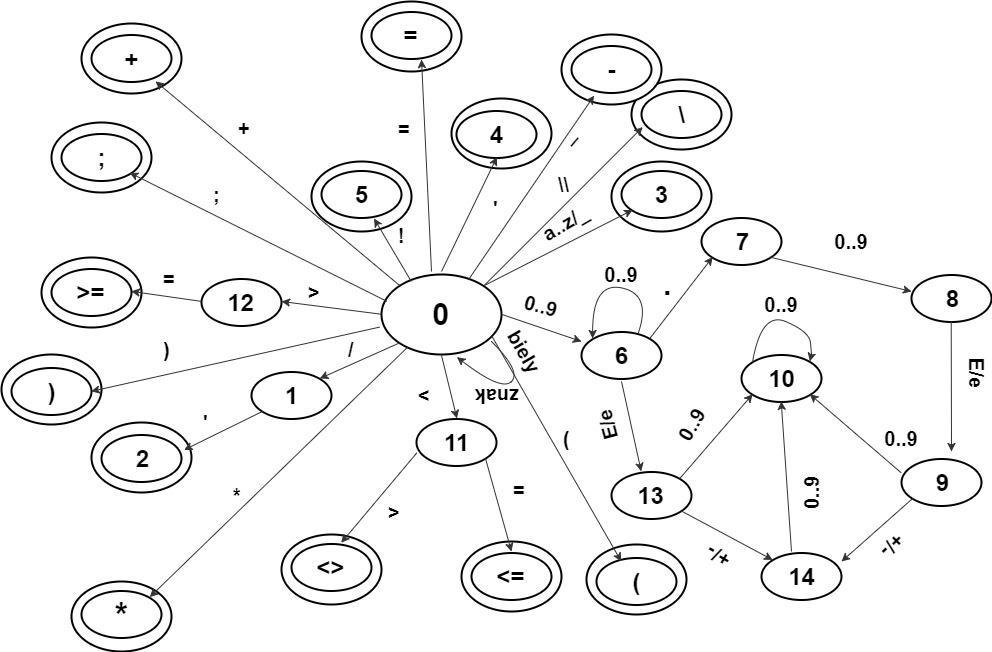
\includegraphics[width=0.7\textwidth]{ka}	
		\caption{Konečný automat}
		\label{ka}
	\end{center}
		\end{figure}	

 \begin{figure} [h]
	\begin{center}
		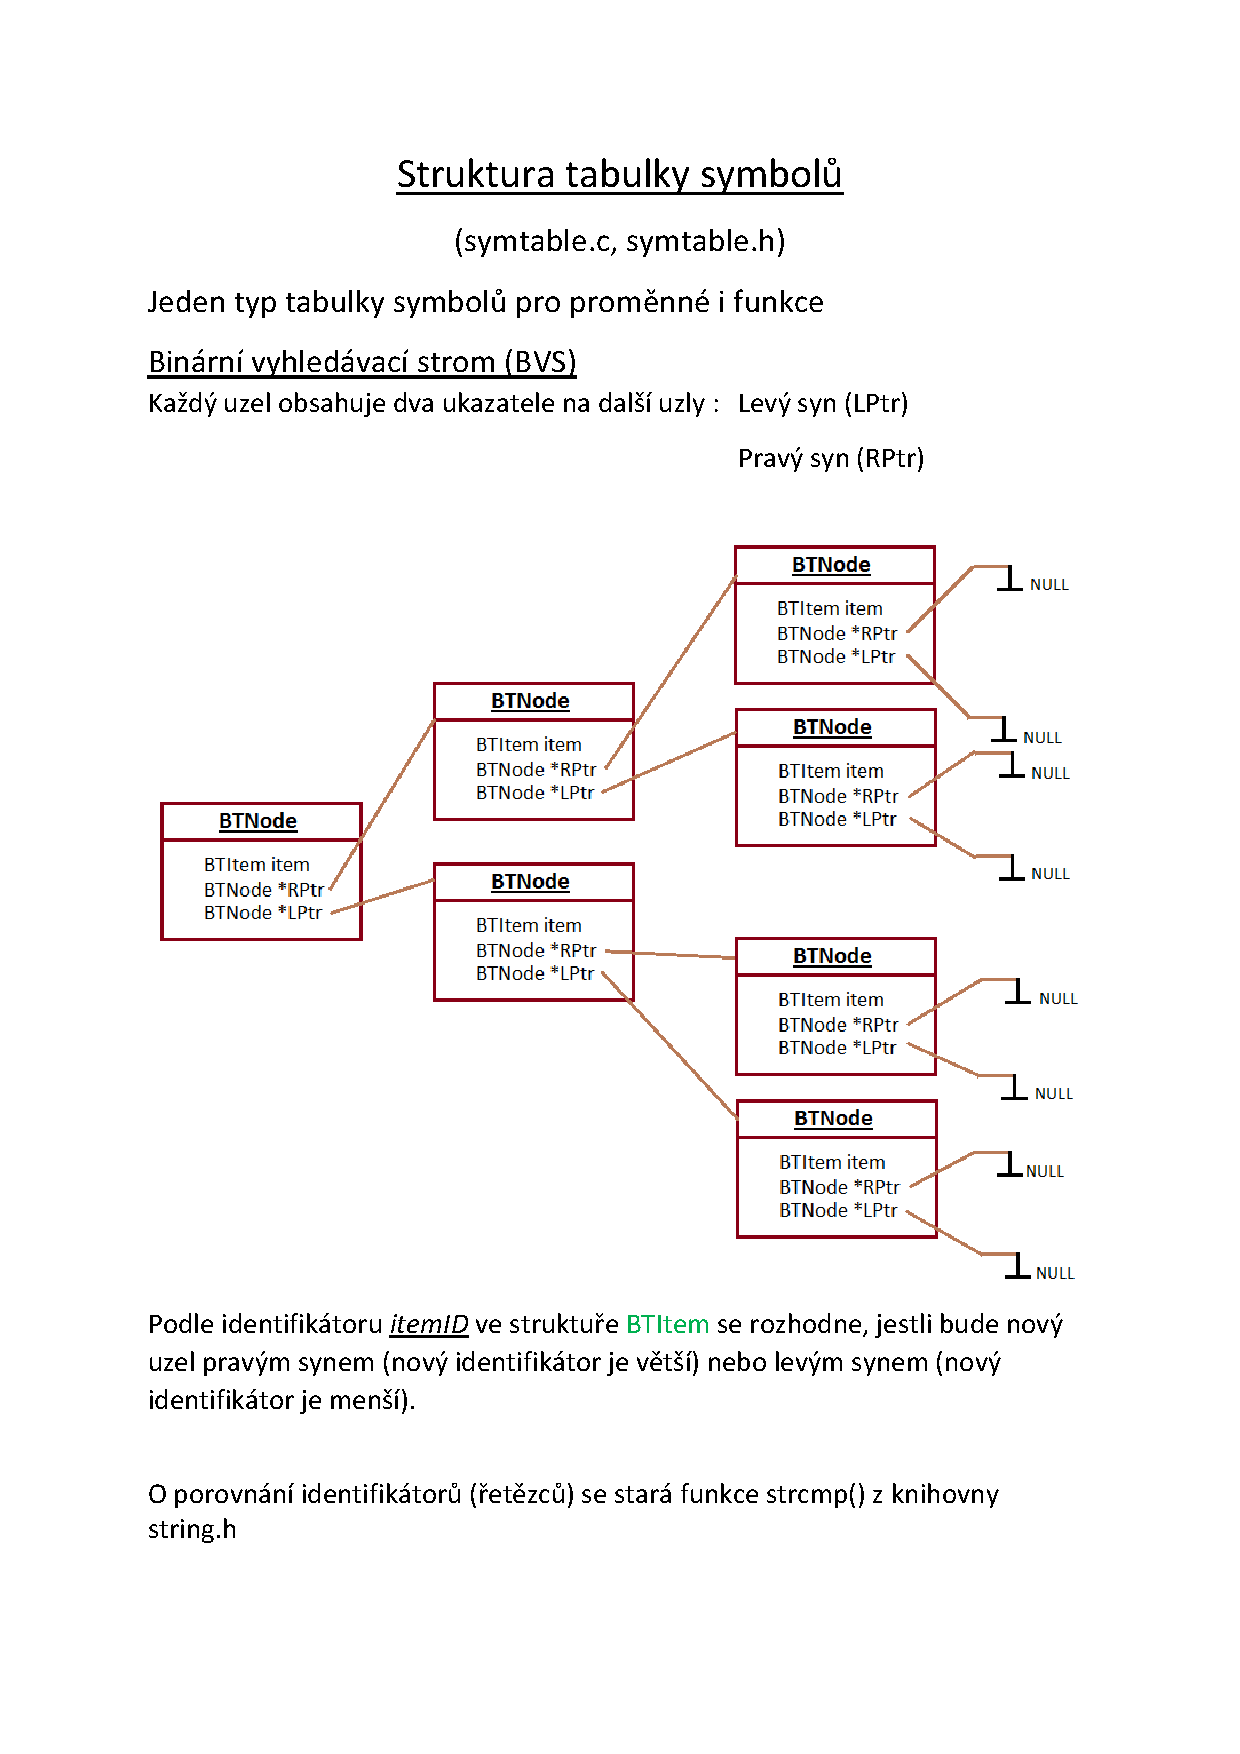
\includegraphics[width=0.8\textwidth]{symtable}	
		\caption{Symtable}
		\label{symtable}
	\end{center}
		\end{figure}	
\begin{figure}[h]
		\begin{center}
			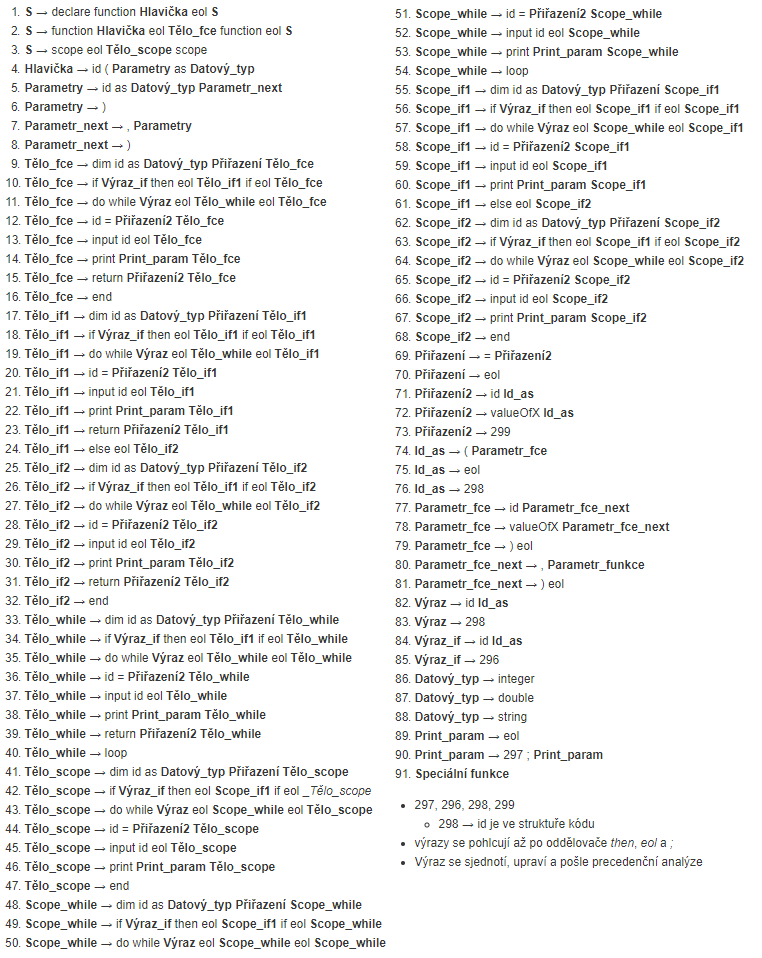
\includegraphics[width=0.99\textwidth]{ll}
			\caption{LL-gramatika}
			\label{ll}
		\end{center}
		\end{figure}
		
			\begin{table}[h]
			\centering
			{\scriptsize {\renewcommand{\arraystretch}{1.2}
			\addtolength{\tabcolsep}{-1.1pt}
			\begin{tabular}{|c|c|c|c|c|c|c|c|c|c|c|c|c|c|c|c|c|c|c|c|c|c|c|}
				\hline
				& D & F & S & id & )  & ,  & dim & if & do & I & P & R & end & E & L & =  & eol & V & int & str & dbl & (  \\ \hline
				S                   & 1       & 2        & 3     &    &    &    &     &    &    &       &       &        &     &      &      &    &     &         &         &        &        &    \\ \hline
				Hlavička            &         &          &       & 4  &    &    &     &    &    &       &       &        &     &      &      &    &     &         &         &        &        &    \\ \hline
				Parametry           &         &          &       & 5  & 6  &    &     &    &    &       &       &        &     &      &      &    &     &         &         &        &        &    \\ \hline
				Parametr\_next      &         &          &       &    & 8  & 7  &     &    &    &       &       &        &     &      &      &    &     &         &         &        &        &    \\ \hline
				Tělo\_fce           &         &          &       & 12 &    &    & 9   & 10 & 11 & 13    & 14    & 15     & 16  &      &      &    &     &         &         &        &        &    \\ \hline
				Tělo\_if1           &         &          &       & 20 &    &    & 17  & 18 & 19 & 21    & 22    & 23     &     & 24   &      &    &     &         &         &        &        &    \\ \hline
				Tělo\_if2           &         &          &       & 28 &    &    & 25  & 26 & 27 & 29    & 30    & 31     & 32  &      &      &    &     &         &         &        &        &    \\ \hline
				Tělo\_while         &         &          &       & 36 &    &    & 33  & 34 & 35 & 37    & 38    & 39     &     &      & 40   &    &     &         &         &        &        &    \\ \hline
				Tělo\_scope         &         &          &       & 44 &    &    & 41  & 42 & 43 & 45    & 46    &        & 47  &      &      &    &     &         &         &        &        &    \\ \hline
				Scope\_while        &         &          &       & 51 &    &    & 48  & 49 & 50 & 52    & 53    &        &     &      & 54   &    &     &         &         &        &        &    \\ \hline
				Scope\_if1          &         &          &       & 58 &    &    & 55  & 56 & 57 & 59    & 60    &        &     & 61   &      &    &     &         &         &        &        &    \\ \hline
				Scope\_if2          &         &          &       & 65 &    &    & 62  & 63 & 64 & 66    & 67    &        & 68  &      &      &    &     &         &         &        &        &    \\ \hline
				Přiřazení           &         &          &       &    &    &    &     &    &    &       &       &        &     &      &      & 69 & 70  &         &         &        &        &    \\ \hline
				Přiřazení2          &         &          &       & 71 &    &    &     &    &    &       &       &        &     &      &      &    &     & 72      &         &        &        &    \\ \hline
				Id\_as              &         &          &       &    &    &    &     &    &    &       &       &        &     &      &      &    & 75  &         &         &        &        & 74 \\ \hline
				Parametr\_fce       &         &          &       & 77 & 79 &    &     &    &    &       &       &        &     &      &      &    &     & 78      &         &        &        &    \\ \hline
				Parametr\_fce\_next &         &          &       &    & 81 & 80 &     &    &    &       &       &        &     &      &      &    &     &         &         &        &        &    \\ \hline
				Výraz               &         &          &       & 82 &    &    &     &    &    &       &       &        &     &      &      &    &     &         &         &        &        &    \\ \hline
				Výraz\_if           &         &          &       & 84 &    &    &     &    &    &       &       &        &     &      &      &    &     &         &         &        &        &    \\ \hline
				Datový\_typ         &         &          &       &    &    &    &     &    &    &       &       &        &     &      &      &    &     &         & 86      & 87     & 88     &    \\ \hline
				Print\_param        &         &          &       &    &    &    &     &    &    &       &       &        &     &      &      &    & 89  &         &         &        &        &    \\ \hline
				\multicolumn{23}{c}{D = declare | F = function | S = scope | V = valueOfX | I = input | P = print | R = return | E = else | L = loop }
			\end{tabular}
			}}
			\caption{LL tabulka}
			\label{gramatika}
		\end{table}
 \begin{figure}[h]
		\begin{center}
		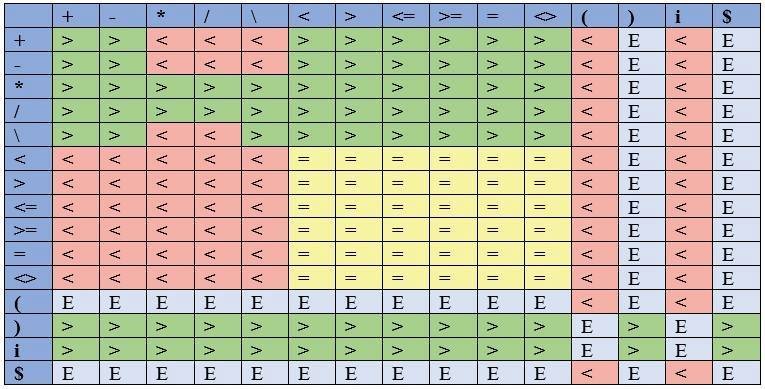
\includegraphics[width=0.99\textwidth]{precedencna}
		\caption{Precedenčná tabuľka}	
		\label{precedencna}
		\end{center}
		\end{figure}	
 
\end{document}
